\documentclass{article}
\usepackage{fontspec}
\usepackage{xeCJK}
\usepackage{amsmath} % 数学公式支持
\usepackage{amsthm}  % 定理环境支持
\newtheorem{theorem}{Theorem}
\usepackage{graphicx}
\usepackage{tikz}
\usetikzlibrary{arrows.meta,3d}

% 中文字体设置
\setCJKmainfont{SimSun} % 宋体
\setCJKsansfont{SimHei} % 黑体
\setCJKmonofont{FangSong} % 仿宋

% 设置段落缩进和行距
\setlength{\parindent}{2em}
\setlength{\parskip}{1em}

\title{离散数学学期课程作业}
\author{离散数学第五小组}
\date{\today}

\begin{document}

\maketitle

\section{引言}


    在数学和计算机科学领域,等价关系作为一种满足自反性、对称性和传递性的二元关系,是将集合元素划分为等价类的理论基础。
等价关系的应用贯穿于众多领域,例如数论中的同余、逻辑中的等价公式以及图论中的节点划分等,
展现了其强大的问题简化能力。在计算机科学中,等价关系常被用来优化算法、压缩状态空间以及提升系统效率。

    本文以确定性有限自动机(Deterministic Finite Automaton, DFA)的状态最小化问题为切入点,
系统性地介绍等价关系的定义与性质,分析其在多个领域中的典型应用,并以 DFA 最小化为案例,
详细讲解如何利用等价关系划分状态集合,实现自动机的简化构造。通过理论与实践相结合,
本文旨在为读者提供理解等价关系及其应用的完整视角。

\newpage
\section{理论基础}
\subsection{等价关系的定义与性质}
    等价关系是一种二元关系$R$,若集合$A$上的二元关系$A$满足以下三个条件,称$\mathrm{R}$为等价关系:
\begin{enumerate}
    \item \textbf{自反性}: $\forall a \in A, (a,a) \in R$
    \item \textbf{对称性}: $\forall (a,b)\in R \rightarrow (b,a) \in R $
    \item \textbf{传递性}: $\forall a,b,c \in A, (a,b) \in R \wedge (b,c) \in R \rightarrow (a,c) \in R$
\end{enumerate}
\subsection{等价类与商集}
在等价关系 $\mathrm{R}$下,集合 $\mathrm{A}$可被划分为若干互不相交的等价类,
每个元素所属的等价类是其在 $\mathrm{R}$下的“等价群体”。
等价类的集合称为商集,记作$\mathrm{A}/\mathrm{R}$。这种划分为解决复杂问题提供了重要的结构化手段。

\subsection{应用意义}
等价关系通过将集合元素划分为等价类,减少了问题的复杂度。在许多算法中,等价关系作为划分与合并的理论基础,为优化问题提供了强有力的支持。


\newpage
\section{等价关系的应用}
\subsection{数学领域}
同余关系:模运算中,整数在模 
$n$ 意义下形成的等价类,即同余类,是数论的基础工具之一。
\subsection{计算机科学领域}
状态最小化:DFA 最小化是等价关系在计算机科学中的经典应用之一,通过等价类划分实现状态压缩。
并查集:用于动态维护元素间等价关系的数据结构,广泛应用于图算法中,如最小生成树的构造。

\subsection{其他领域}
逻辑与推理:等价公式的判定与简化。
网络科学:在社交网络中分析等价节点的聚类特性。


\newpage
\section{等价关系在DFA中的应用}
\subsection{背景介绍}
    \textbf{DFA(deterministic finite automaton)}是一个有限状态机,通过接受由字符串唯一确定的状态序列来接受或拒绝给定的字符串
    \textbf{有限状态自动机}$M$是一个五元组$(Q, \Sigma, \delta, q_0, F)$,包含了
    \begin{itemize}
        \item 有限状态$Q$
        \item 有限输入符号$\Sigma$
        \item 转移函数$\delta: Q \times \Sigma \mapsto Q$
        \item 初识状态$q_0$
        \item 可接受状态集合$F \subset Q$
    \end{itemize}
    当一个字符串$w = a_0a_1\cdots a_n$输入状态机中,称$w$是可接受的当且仅当状态机接受$w$后产生的序列$r_0, r_1, \cdots, r_n$满足:
    \begin{enumerate}
        \item $r_0 = q_0$
        \item $r_{k+1} = \delta(r_k, q_k+1), for k = 0, 1, \ldots, n-1$
        \item $r_n \in F$
    \end{enumerate}
    称所有可接受的字符串为有限状态机$M$的语言,记为$L(M)$。
    
    其中$\delta$通常用状态转移表和状态转移图表示, 下面以一个$M_1$为例子
    \begin{figure}[h]
        \centering
        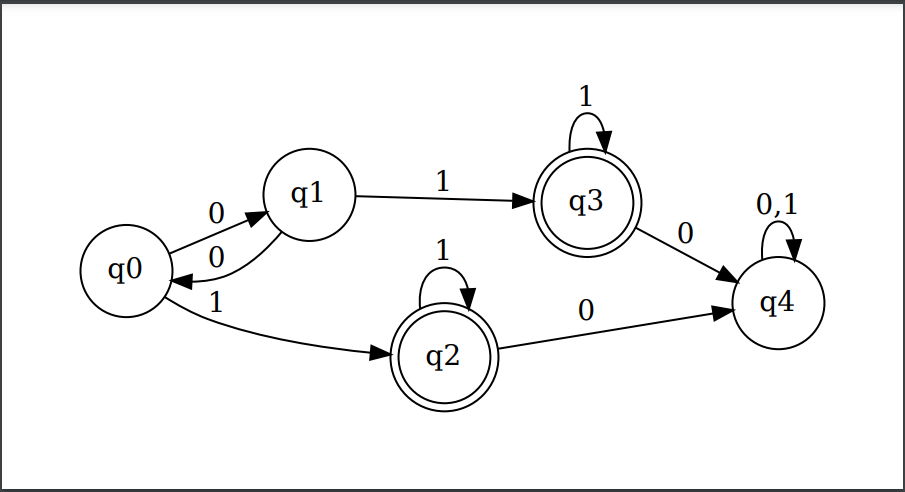
\includegraphics[scale=0.2]{Img/dfa_example.png}
        \caption{有限状态机$M_1$的状态转移图}
    \end{figure}
    在有限状态机$M_1$中, $Q=\{q_0, q_1,q_2,q_3,q_4\}$, $\Sigma = \{0,1\}$, 初始状态为$q_0$
    可接受状态的集合$F = \{q_2, q_3\}$, 其中状态转移图由双圆圈标出的状态为可接受状态


\subsection{等价关系在DFA中的应用}

\subsection{DFA最小化意义}


\subsection{DFA最小化方法}
    状态最小化一般分为两个步骤:
    \textbf{步骤一}
    首先,将 DFA 的所有状态分成两组:
    \begin{itemize}
        \item 结束状态(接受信号并输出结果的状态)。
        \item 非结束状态(不会输出结果的状态)。 
    \end{itemize}
    这两组不可能是相同的,因为它们在 DFA 中执行的功能显然不同。   

    \textbf{步骤二}
    然后,重复涉及 DFA 的所有状态,根据它们在接收信号后的转移情况进一步分组。举一个简单的示例:
    \begin{itemize}
        \item 如果状态 A 和 B 在接收同样的信号后,转向了同一组的其他状态,那么 A 和 B 可以视为相同状态,将它们合并。
        \item 如果不同,则它们需要分在不同组中。
    \end{itemize}
    这个过程是通过一种迭代方式完成的,直到没有更多的状态需要分组。

    \textbf{步骤三}
    最后,根据分组结果,将同一组的状态合并为一个新状态,构造出一个最小化后的 DFA。
    

\subsection{DFA最小化算法}
\subsubsection{Hopcraft算法}
    这部分由陈新宇完成
\subsubsection{常翰堃算法(bushi)}
    这部分由常翰堃完成


\newpage
\section{总结}




\newpage
\section{参考文献}
\begin{enumerate}
    \item Hopcroft, J.E.Motwani, R.Ullman, J.D.(2007). $Introduction to Automata Theory, Languages, and Computation.$
    \item Sipser.M.(2013). $Introduction to the Theory of Computation. Cengage Learning.$
\end{enumerate}


\end{document}